\section{计算几何}

\subsection{二维几何基础库（base.hpp）}

\begin{lstlisting}
#include <bits/stdc++.h>
using namespace std;
using ll = long long;
using ld = long double;
using Real = long double;
using i128 = __int128;
constexpr Real PI = numbers::pi;
constexpr Real EPS = 1e-8;

inline int sgn(Real x) {
    return (x > EPS) - (x < -EPS);
}
inline int sgn(ll x) {
    return (x > 0) - (x < 0);
}

inline int cmp(Real x, Real y) {
    return sgn(x - y);
}
inline int cmp(ll x, ll y) {
    return (x > y) - (x < y);
}

inline Real arccos(Real c) {
    c = max(c, Real(-1.0));
    c = min(c, Real(1.0));
    return acosl(c);
}

template <class T>
struct Pnt {
    T x, y;
    Pnt(T x = 0, T y = 0) : x(x), y(y) {}
    template <class U> operator Pnt<U>() const {
        return Pnt<U>(U(x), U(y));
    }

    Pnt& operator+=(const Pnt& o) & {
        return x += o.x, y += o.y, *this;
    }
    Pnt& operator-=(const Pnt& o) & {
        return x -= o.x, y -= o.y, *this;
    }
    Pnt& operator*=(T o) & {
        return x *= o, y *= o, *this;
    }
    Pnt& operator/=(T o) & {
        return x /= o, y /= o, *this;
    }
    Pnt operator-() const {
        return Pnt(-x, -y);
    }

    friend Pnt operator+(Pnt a, const Pnt& b) {
        return a += b;
    }
    friend Pnt operator-(Pnt a, const Pnt& b) {
        return a -= b;
    }
    friend Pnt operator*(Pnt a, T b) {
        return a *= b;
    }
    friend Pnt operator*(T a, Pnt b) {
        return b *= a;
    }
    friend Pnt operator/(Pnt a, T b) {
        return a /= b;
    }
    bool operator<(const Pnt& o) const {
        if (x != o.x) return x < o.x;
        return y < o.y;
    }
    bool operator>(const Pnt& o) const {
        return o < *this;
    }
    bool operator==(const Pnt& o) const {
        return (cmp(x, o.x) == 0) && (cmp(y, o.y) == 0);
    }
    bool operator!=(const Pnt& o) const {
        return !(*this == o);
    }
    friend istream& operator>>(istream& is, Pnt<T>& p) {
        return is >> p.x >> p.y;
    }
    friend ostream& operator<<(ostream& os, const Pnt<T>& p) {
        return os << '(' << p.x << ", " << p.y << ')';
    }
};
using Pr = Pnt<Real>;
#define Pt Pnt<T>

template <class T>
T dot(const Pt& a, const Pt& b) {
    return a.x * b.x + a.y * b.y;    
}
template <class T>
T dot(const Pt& o, const Pt& a, const Pt& b) {
    return dot(a - o, b - o);
}

template <class T>
T crs(const Pt& a, const Pt& b) {
    return a.x * b.y - a.y * b.x;
}
template <class T>
T crs(const Pt& o, const Pt& a, const Pt& b) {
    return crs(a - o, b - o);
}

inline i128 crs128(const Pnt<ll>& a, const Pnt<ll>& b) {
    return (i128)a.x * b.y - (i128)a.y * b.x;
}
inline i128 dot128(const Pnt<ll>& a, const Pnt<ll>& b) {
    return (i128)a.x * b.x + (i128)a.y * b.y;
}


template <typename T>
T len2(const Pt& p) {
    return dot(p, p);
}
inline Real len(const Pr& p) {
    return sqrtl(len2(p));
}

template <typename T>
T dis2(const Pt& a, const Pt& b) {
    return dot(a - b, a - b);
}
inline Real dis(const Pr& a, const Pr& b) {
    return sqrtl(dis2(a, b));
}

template <class T>
T manhattan(const Pt& a, const Pt& b) {
    return abs(a.x - b.x) + abs(a.y - b.y);
}

inline Pr norm(Pr a) {
    // 非零
    return a / len(a);
}

inline Real agl(const Pr& a, const Pr& b) {
    // 需保证非零
    Real val = fabsl(crs(a, b));
    return fabsl(atan2l(val, dot(a, b)));
}

inline Real agl(Real a, Real b, Real c) {
    // 余弦定理
    return arccos((a * a + b * b - c * c) / (2.0 * a * b));
}

inline Pr rotate(const Pr& a, Real theta) {
    Real c = cosl(theta), s = sinl(theta);
    return Pr(c * a.x - s * a.y, s * a.x + c * a.y);
}
inline Pr rotate(const Pr& o, const Pr& a, Real theta) {
    // a 绕 o 转 theta
    return o + rotate(a - o, theta);
}

template <class T>
Pt perp(const Pt& a) {
    return { -a.y, a.x };
}
template <class T>
Pt perp(const Pt& o, const Pt& a) {
    return o + perp(a - o);
}

inline Real toDeg(Real x) {
    // 转角度
    return x * 180 / PI;
}
inline Real toArc(Real x) {
    // 转弧度
    return PI / 180 * x;
}


template <typename T>
struct Seg {
    Pt a, b;
    Seg(const Pt& a = {}, const Pt& b = {}) : a(a), b(b) {}
    template<class U> operator Seg<U>() const { // 自动类型匹配
        return Seg<U>(Pnt<U>(a), Pnt<U>(b));
    }
};
#define St Seg<T>
using Sr = Seg<Real>;

template <class T>
struct Lin {
    Pt p, v;
    Lin(Pt p = {}, Pt v = {}) : p(p), v(v) {}
    Lin(const St& s) : p(s.a), v(s.b - s.a) {}
    template<class U> operator Lin<U>() const { // 自动类型匹配
        return Lin<U>(Pnt<U>(p), Pnt<U>(v));
    }
};
#define Lt Lin<T>
using Lr = Lin<Real>;

enum Relation { 
    ONBACK = -2, 
    CW, // clockwise
    ON,
    CCW, // counter-clockwise
    ONFRONT
};

template <class T>
int rls(const Pt& p, const Lt& l) { // relation
    return sgn(crs(l.v, p - l.p));
}

template <class T>
int rls(const Pt& p, const St& s) {
    int tmp = rls(p, Lin(s));
    if (tmp != 0) {
        return tmp;
    }
    if (sgn(dot(s.a, s.b, p)) < 0) {
        return ONBACK;
    } else if (sgn(dot(s.b, s.a, p)) < 0) {
        return ONFRONT;
    }
    return ON;
}

inline Pr project(const Pr& p, const Lr& l) {
    // 需保证l.v非零
    Pr t = l.v * dot(p - l.p, l.v);
    return l.p + t / len2(l.v);
}

inline Pr reflect(const Pr& p, const Lr& l) {
    return project(p, l) * 2 - p;
}

template <class T>
bool parallel(const Pt& a, const Pt& b) {
    return sgn(crs(a, b)) == 0;
}
template <class T>
bool orthogonal(const Pt& a, const Pt& b) {
    return sgn(dot(a, b)) == 0;
}


// 线段相交, 快速排斥实验
template <class T>
bool box_joint(const St& a, const St& b) { // 快速排斥实验
    Pt A = { a.a.x, a.a.y }, 
        B = { a.b.x, a.b.y }, 
        C = { b.a.x, b.a.y },
        D = { b.b.x, b.b.y };
    return 
        cmp(min(A.x, B.x), max(C.x, D.x)) <= 0 && 
        cmp(min(C.x, D.x), max(A.x, B.x)) <= 0 && 
        cmp(min(A.y, B.y), max(C.y, D.y)) <= 0 && 
        cmp(min(C.y, D.y), max(A.y, B.y)) <= 0;
}

// 跨立实验
template <class T>
bool straddle(const St& a, const St& b) {
    return sgn(crs(a.a, a.b, b.a)) * sgn(crs(a.a, a.b, b.b)) <= 0;
}

template <class T>
bool intersect(const St a, const St& b) {
    return box_joint(a, b) && 
           straddle(a, b) && 
           straddle(b, a);
}

// 直线相交
template <class T>
inline bool intersect(const Lt& a, const Lt& b) {
    if (sgn(crs(a.v, b.v)) != 0) {
        return true;
    } else {
        return sgn(crs(a.v, b.p - a.p)) == 0;
    }
}

// 直线交点
inline Pr intersection(const Lr& a, const Lr& b) {
    // 需保证不平行
    assert(sgn(crs(a.v, b.v)) != 0);
    return a.p + a.v * crs(b.p - a.p, b.v) / crs(a.v, b.v);
}

// 点-直线距离
inline Real dist(const Pr& a, const Lr& l) {
    return fabsl(crs(l.v, a - l.p) / len(l.v));
}
// 点-线段距离
inline Real dist(const Pr& p, const Sr& s) {
    Pr ab = s.b - s.a, 
       ap = p - s.a, 
       ba = s.a - s.b,
       bp = p - s.b;
    if (sgn(dot(ab, ap)) < 0) {
        return len(ap);
    } else if (sgn(dot(ba, bp)) < 0) {
        return len(bp);
    }
    return fabsl(crs(ab, ap)) / len(ab);
}

// 线段-线段距离
inline Real dist(const Sr& a, const Sr& b) {
    if (intersect(a, b)) {
        return 0;
    }
    return min({ 
        dist(a.a, b),
        dist(a.b, b),
        dist(b.a, a),
        dist(b.b, a)
    });
}

template <class T>
using Polygon = vector<Pnt<T>>; // 需要保证逆时针存储
inline Real area(const Polygon<Real>& pol) {
    Real ret = 0;
    int n = pol.size();
    for (int i = 0; i < n; i++) {
        ret += crs(pol[i], pol[(i + 1) % n]);
    }
    return abs(ret) / 2;
}

enum Inside {
    OUT = 0,
    ONSEG,
    IN
};
template <class T>
inline int inside(const Pt& p, const Polygon<T>& pol) {
    int wn = 0;
    int n = pol.size();
    
    for (int i = 0; i < n; i++) {
        const auto& v1 = pol[i];
        const auto& v2 = pol[(i + 1) % n];
        if (rls(p, Seg(v1, v2)) == ON) {
            return ONSEG;
        }
        int s1 = sgn(v1.y - p.y);
        int s2 = sgn(v2.y - p.y);
        int s3 = sgn(crs(v2 - v1, p - v1));
        if (s1 <= 0) {
            if (s2 > 0 && s3 > 0) {
                wn++;
            }
        } else {
            if (s2 <= 0 && s3 < 0) {
                wn--;
            }
        }
    }
    if (wn != 0) {
        return IN;
    } else {
        return OUT;
    }
}

inline int inside(const Sr& s, const Polygon<Real>& pol) {
    if (inside(s.a, pol) * inside(s.b, pol) == 0) {
        return OUT;
    }
    int n = pol.size();
    for (int i = 0; i < n; i++) {
        const auto& p1 = pol[i];
        const auto& p2 = pol[(i + 1) % n];
        Seg edge(p1, p2);
        if (sgn(crs(s.b - s.a, edge.a - s.a)) * sgn(crs(s.b - s.a, edge.b - s.a)) < 0 &&
            sgn(crs(edge.b - edge.a, s.a - edge.a)) * sgn(crs(edge.b - edge.a, s.b - edge.a)) < 0) {
            return OUT;
        }
    }
    
    vector<Pr> pts;
    pts.emplace_back(s.a);
    pts.emplace_back(s.b);
    for (int i = 0; i < n; i++) {
        if (rls(pol[i], s) == ON) {
            pts.emplace_back(pol[i]);
        }
    }
    auto param = [&](const Pr& p) -> Real {
        Pr v = s.b - s.a;
        if (fabsl(v.x) >= fabsl(v.y)) {
            return (p.x - s.a.x) / v.x;
        } else {
            return (p.y - s.a.y) / v.y;
        }
    };
    sort(pts.begin(), pts.end(), [&](const Pr& u, const Pr& v) {
        return param(u) < param(v);
    });
    pts.erase(unique(pts.begin(), pts.end()), pts.end());

    bool flag = false;
    for (const auto& p : pts) {
        if (inside(p, pol) == ONSEG) {
            flag = true;
        }
    }
    for (int i = 0; i + 1 < (int)pts.size(); i++) {
        if (pts[i] == pts[i + 1]) {
            continue;
        }
        Pr mid = (pts[i] + pts[i + 1]) / 2;
        int t = inside(mid, pol);
        if (t == OUT) {
            return OUT;
        }
    }

    if (flag) {
        return ONSEG;
    }
    return IN;
}

template <class T>
inline bool is_convex(const Polygon<T>& pol) {
    // 允许相邻边共线
    int n = pol.size();
    Pt v1;
    Pt v2 = pol[1] - pol[0];
    for (int i = 1; i < n; i++) {
        v1 = v2;
        v2 = pol[(i + 1) % n] - pol[i];
        if (sgn(crs(v1, v2)) < 0) {
            return false;
        }
    }
    return true;
}

// 1 : 上半, 0 : 原点, -1 : 下半
template <class T>
inline int up_dn(const Pt& p) {
    if (sgn(p.y) == 0) {
        return sgn(p.x);
    }
    return sgn(p.y);
}

template <class T>
inline int polar_cmp(const Pt& lt, const Pt& rt) {
    int a = up_dn(lt), b = up_dn(rt);
    if (a != b) {
        return (a < b) ? -1 : 1;
    }
    auto c = crs(lt, rt);
    return -sgn(c);
}

struct Circle {
    Pr o;
    Real r;
};



#undef Pt
#undef Pr
#undef St
#undef Sr
#undef Lt
#undef Lr
\end{lstlisting}

\subsection{极角排序}

\begin{lstlisting}
#include "base.hpp"
template <class S> 
int halfPlane(Pnt<S> a) {
    if (cmp(a.y, 0) == 0) {
        return cmp(a.x, 0);
    }
    return cmp(a.y, 0); // 如果需要从负半轴开始则把这里改成负的
}
template <class S>
bool polarCmp(Pnt<S> a, Pnt<S> b) {
    if (halfPlane(a) != halfPlane(b)) {
        return halfPlane(a) > halfPlane(b);
    }
    if (sgn(crs(a, b)) == 0) {
        return len2(a) < len2(b);
    }
    return sgn(crs(a, b)) > 0;
}
\end{lstlisting}

\subsection{平面几何杂项（sgn / cmp / 读入）}

\begin{lstlisting}
// 平面几何杂项（CG.md「平面几何必要初始化」中 base.hpp 未覆盖的部分）
// 依赖 base.hpp：Real / EPS / sgn / cmp
#include "base.hpp"

// 实数域 gcd（CG.md: fgcd(ld x, ld y)）
inline Real fgcd(Real x, Real y) {
    return fabsl(y) < EPS ? fabsl(x) : fgcd(y, fmodl(x, y));
}

// 近似相等（等价于 cmp(x, y) == 0）
// CG.md: equal(T x, S y)
template <class T, class S>
inline bool equal(T x, S y) {
    return -EPS < x - y && x - y < EPS;
}

// 字符串读入浮点数：截断到 k 位小数后转为整数（放大 10^k 倍）
// 定点化之后就能用整数精确运算，避免浮点误差。CG.md: read(int k = Knum)
inline ll readReal(int k = 4) {
    string s;
    cin >> s;

    int num = 0;
    int it = (int)s.find('.');
    if (it != -1) {                   // 存在小数点
        num = (int)s.size() - it - 1; // 计算小数位数
        s.erase(s.begin() + it);      // 删除小数点
    }
    if (num > k) {                       // 小数位过多时截断（原文档未处理这种情况）
        s.erase(s.size() - (num - k));   // 删掉末尾多余的 num - k 位
        num = k;
    }
    for (int i = 1; i <= k - num; i++) { // 补全小数位数
        s += '0';
    }
    return stoll(s);
}
\end{lstlisting}

\subsection{平面点线运算}

\begin{lstlisting}
// 平面点线补充（CG.md「平面点线相关」中 base.hpp 未覆盖的部分）
// 依赖 base.hpp
#include "base.hpp"
// 注：点在直线/线段上、垂足、距离、平行垂直等 base.hpp 已提供，见 rls / project / dist / parallel / orthogonal

// 线段的中垂线（垂直平分线）（CG.md: midSegment）
inline Lr midSegment(const Sr& l) {
    Pr mid = (l.a + l.b) / 2; // 线段中点
    return Lr(mid, perp(l.b - l.a));
}

// 点到直线的最近点与最近距离，返回 {最近点, 最近距离}（CG.md: pointToLine）
inline pair<Pr, Real> pointToLine(const Pr& p, const Lr& l) {
    Pr ans = project(p, l);
    return {ans, dis(p, ans)};
}

// 点到线段的最近点与最近距离，返回 {最近点, 最近距离}（CG.md: pointToSegment）
inline pair<Pr, Real> pointToSegment(const Pr& p, const Sr& s) {
    if (sgn(dot(s.a, p, s.b)) < 0) {        // 垂足落在 a 端外侧，最近点是 a
        return {s.a, dis(p, s.a)};
    } else if (sgn(dot(s.b, p, s.a)) < 0) { // 垂足落在 b 端外侧，最近点是 b
        return {s.b, dis(p, s.b)};
    }
    return pointToLine(p, Lr(s));
}

// 点相对直线的方位：1 左侧(逆时针)，0 直线上，-1 右侧
template <class T>
inline int lineSide(const Pnt<T>& p, const Lin<T>& l) {
    return sgn(crs(l.v, p - l.p));
}

// 两点是否在直线同侧 / 异侧（有任一点落在直线上时都返回 false）
// CG.md: pointOnLineSide / pointNotOnLineSide
// 原文档用两个叉乘相乘再取符号，这里先取符号再相乘，避免整数溢出
template <class T>
inline bool pointOnLineSide(const Pnt<T>& p1, const Pnt<T>& p2, const Lin<T>& l) {
    return lineSide(p1, l) * lineSide(p2, l) == 1;
}
template <class T>
inline bool pointNotOnLineSide(const Pnt<T>& p1, const Pnt<T>& p2, const Lin<T>& l) {
    return lineSide(p1, l) * lineSide(p2, l) == -1;
}

// 两线段是否相交及交点（扩展版，可以处理共线重叠）
// 返回 {type, p1, p2}：0 不相交；1 普通相交；2 重叠（交于两点）；3 相交于端点
// CG.md: segmentIntersection（返回交点的那一版，务必用浮点）
inline tuple<int, Pr, Pr> segmentIntersection(const Sr& l1, const Sr& l2) {
    auto [s1, e1] = l1;
    auto [s2, e2] = l2;
    Real A = max(s1.x, e1.x), AA = min(s1.x, e1.x);
    Real B = max(s1.y, e1.y), BB = min(s1.y, e1.y);
    Real C = max(s2.x, e2.x), CC = min(s2.x, e2.x);
    Real D = max(s2.y, e2.y), DD = min(s2.y, e2.y);
    if (A < CC || C < AA || B < DD || D < BB) { // 快速排斥实验
        return {0, {}, {}};
    }
    if (sgn(crs(e1 - s1, e2 - s2)) == 0) { // 平行
        if (sgn(crs(s1, s2, e1)) != 0) {   // 不共线
            return {0, {}, {}};
        }
        Pr p1(max(AA, CC), max(BB, DD));
        Pr p2(min(A, C), min(B, D));
        if (rls(p1, l1) != ON) { // 修正端点顺序
            swap(p1.y, p2.y);
        }
        if (p1 == p2) {
            return {3, p1, p2};
        }
        return {2, p1, p2};
    }
    Real cp1 = crs(s2 - s1, e2 - s1);
    Real cp2 = crs(s2 - e1, e2 - e1);
    Real cp3 = crs(s1 - s2, e1 - s2);
    Real cp4 = crs(s1 - e2, e1 - e2);
    if (sgn(cp1 * cp2) == 1 || sgn(cp3 * cp4) == 1) { // 跨立实验不通过
        return {0, {}, {}};
    }
    Pr p = intersection(Lr(l1), Lr(l2)); // 需要浮点
    if (sgn(cp1) != 0 && sgn(cp2) != 0 && sgn(cp3) != 0 && sgn(cp4) != 0) {
        return {1, p, p};
    }
    return {3, p, p};
}
\end{lstlisting}

\subsection{平面直线方程转换}

\begin{lstlisting}
// 平面直线方程转换（CG.md「平面直线方程转换」全节）
// 依赖 base.hpp
#include "base.hpp"

// 浮点斜率：注意平行于 y 轴时结果为 inf（CG.md: slope）
inline Real slope(const Pr& p1, const Pr& p2) {
    return (p1.y - p2.y) / (p1.x - p2.x);
}
inline Real slope(const Lr& l) {
    return slope(l.p, l.p + l.v);
}

// 分数精确斜率：返回最简分数 {分子, 分母}，分母恒正；平行于 y 轴时返回 {1, 0}
// CG.md 用 Frac<T> 实现（本仓库没有分数类，这里直接返回约分后的分子分母）
// 仅适用于整数类型
template <class T>
inline pair<T, T> slopeEx(const Pnt<T>& p1, const Pnt<T>& p2) {
    T u = p1.y - p2.y, v = p1.x - p2.x;
    if (v == 0) {
        return {1, 0}; // inf
    }
    if (u == 0) {
        return {0, 1};
    }
    T g = gcd(abs(u), abs(v));
    u /= g, v /= g;
    if (v < 0) { // 符号调整，恒保证分母为正
        u = -u, v = -v;
    }
    return {u, v};
}

// 两点式转一般式：返回 {A, B, C}，表示 Ax + By = C
// 可以处理平行于 x, y 轴、两点重合的情况（CG.md: getfun(Lt p)）
// 仅适用于整数类型
template <class T>
inline tuple<T, T, T> getfun(const Pnt<T>& p1, const Pnt<T>& p2) {
    T A = p1.y - p2.y, B = p2.x - p1.x, C = p1.x * A + p1.y * B;
    if (A < 0) { // 符号调整
        A = -A, B = -B, C = -C;
    } else if (A == 0) {
        if (B < 0) {
            B = -B, C = -C;
        } else if (B == 0 && C < 0) {
            C = -C;
        }
    }
    if (A == 0) { // 数值约分
        if (B == 0) {
            C = 0; // 两点重合
        } else {
            T g = gcd(abs(B), abs(C));
            B /= g, C /= g;
        }
    } else if (B == 0) {
        T g = gcd(abs(A), abs(C));
        A /= g, C /= g;
    } else {
        T g = gcd(gcd(abs(A), abs(B)), abs(C));
        A /= g, B /= g, C /= g;
    }
    return {A, B, C}; // Ax + By = C
}

// 一般式转两点式：返回直线上的两个点（用线段类型Seg装），A = B = 0 时不合法
// 整数点可能很大或不存在，故直接采用浮点数；与 x, y 轴有交点时取交点
// （CG.md: getfun(int A, int B, int C)）
inline Sr getfun(ll A, ll B, ll C) {
    Real x1 = 0, y1 = 0, x2 = 0, y2 = 0;
    if (A && B) { // 正常
        if (C) {
            x1 = 0, y1 = (Real)C / B;
            y2 = 0, x2 = (Real)C / A;
        } else { // 过原点
            x1 = 1, y1 = -(Real)A / B;
            x2 = 0, y2 = 0;
        }
    } else if (A && !B) { // 垂直
        if (C) {
            y1 = 0, x1 = (Real)C / A;
            y2 = 1, x2 = x1;
        } else {
            x1 = 0, y1 = 1;
            x2 = 0, y2 = 0;
        }
    } else if (!A && B) { // 水平
        if (C) {
            x1 = 0, y1 = (Real)C / B;
            x2 = 1, y2 = y1;
        } else {
            x1 = 1, y1 = 0;
            x2 = 0, y2 = 0;
        }
    } else { // 不合法，请特判
        assert(false);
    }
    return Sr({x1, y1}, {x2, y2});
}

// 抛物线与 x 轴是否相交及交点：0 没有交点；1 相切；2 有两个交点
// CG.md: getAns(ld a, ld b, ld c)，即 ax^2 + bx + c = 0
inline tuple<int, Real, Real> parabolaRoots(Real a, Real b, Real c) {
    Real delta = b * b - a * c * 4;
    if (delta < 0.) {
        return {0, 0, 0};
    }
    delta = sqrtl(delta);
    Real ans1 = -(delta + b) / 2 / a;
    Real ans2 = (delta - b) / 2 / a;
    if (ans1 > ans2) {
        swap(ans1, ans2);
    }
    if (sgn(delta) == 0) { // 相切
        return {1, ans2, 0};
    }
    return {2, ans1, ans2};
}
\end{lstlisting}

\subsection{平面三角形相关（四心）}

\begin{lstlisting}
// 平面三角形相关（CG.md「平面三角形相关（浮点数处理）」全节）
// 依赖 base.hpp：crs / perp / norm / intersection
#include "base.hpp"
// 说明：三角形面积也可以直接用 base.hpp 的 area(Polygon<Real>)，这里给出三点版本

// 三角形面积（CG.md: area(Point<ld> a, Point<ld> b, Point<ld> c)）
inline Real area(const Pr& a, const Pr& b, const Pr& c) {
    return fabsl(crs(b, c, a)) / 2;
}

// 外心：三边垂直平分线的交点（外接圆圆心）（CG.md: center1）
// 需保证三点不共线
inline Pr circumcenter(const Pr& p1, const Pr& p2, const Pr& p3) {
    Lr u((p1 + p2) / 2, perp(p2 - p1)); // p1p2 的中垂线
    Lr v((p2 + p3) / 2, perp(p3 - p2)); // p2p3 的中垂线
    return intersection(u, v);
}

// 内心：三条内角平分线的交点（内切圆圆心）（CG.md: center2）
// 需保证三点不共线
inline Pr incenter(const Pr& p1, const Pr& p2, const Pr& p3) {
    // 角平分线方向 = 两条边的单位向量之和
    // （原文档用 atan2 取两角度的平均值，跨越 ±π 时会算错方向）
    auto bisector = [](const Pr& o, const Pr& u, const Pr& v) {
        return norm(u - o) + norm(v - o);
    };
    Lr U(p1, bisector(p1, p2, p3));
    Lr V(p2, bisector(p2, p1, p3));
    return intersection(U, V);
}

// 垂心：三条高线所在直线的交点（CG.md: center3）
// 需保证三点不共线
inline Pr orthocenter(const Pr& p1, const Pr& p2, const Pr& p3) {
    Lr U(p1, perp(p2 - p3)); // 过 p1 的高线，垂直于 p2p3
    Lr V(p2, perp(p1 - p3)); // 过 p2 的高线，垂直于 p1p3
    return intersection(U, V);
}
\end{lstlisting}

\subsection{平面圆相关（交点 / 切线 / 相交面积）}

\begin{lstlisting}
// 平面圆相关（CG.md「平面圆相关（浮点数处理）」全节）
// 依赖 base.hpp：project / norm / dis / dis2 / crs / agl / intersection / PI
#include "base.hpp"
// 说明：圆用 base.hpp 里的 Circle{Pr o; Real r;} 或直接传 圆心 + 半径

// 根据圆心角获取圆上某点：把圆上最右侧的点绕圆心逆时针旋转 rad 弧度
// CG.md: getPoint(Point<ld> p, ld r, ld rad)
inline Pr pointOnCircle(const Pr& o, Real r, Real rad) {
    return {o.x + cosl(rad) * r, o.y + sinl(rad) * r};
}

// 点到圆的最近点：返回 {最近点, 最近距离}
// p 为圆心时最近点不唯一，视作输入错误，返回圆心（CG.md: pointToCircle）
inline pair<Pr, Real> pointToCircle(const Pr& p, const Pr& o, Real r) {
    if (sgn(dis(p, o)) == 0) {
        return {o, 0};
    }
    Pr u = o + norm(p - o) * r; // 近端：圆心指向 p 的方向
    Pr v = o - norm(p - o) * r; // 远端
    Real du = dis(u, p), dv = dis(v, p);
    if (du < dv) {
        return {u, du};
    }
    return {v, dv};
}

// 直线是否与圆相交及交点：0 不相交；1 相切；2 相交（CG.md: lineCircleCross）
// 需保证直线的方向向量非零
inline tuple<int, Pr, Pr> lineCircleCross(const Lr& l, const Pr& o, Real r) {
    Pr p = project(o, l);              // 圆心到直线的垂足
    Real tmp = r * r - dis2(p, o);     // 用平方距离，避免开根号
    if (sgn(tmp) < 0) {
        return {0, {}, {}};
    } else if (sgn(tmp) == 0) {
        return {1, p, {}};
    }
    Pr vec = norm(l.v) * sqrtl(tmp);
    return {2, p + vec, p - vec};
}

// 线段是否与圆相交及交点：0 不相交；1 相切于线段上；2 交于一个点；3 交于两个点
// CG.md: segmentCircleCross
inline tuple<int, Pr, Pr> segmentCircleCross(const Sr& l, const Pr& o, Real r) {
    auto [type, U, V] = lineCircleCross(Lr(l), o, r);
    bool f1 = rls(U, l) == ON, f2 = rls(V, l) == ON; // 交点是否落在线段上
    if (type == 1 && f1) {
        return {1, U, {}};
    } else if (type == 2 && f1 && f2) {
        return {3, U, V};
    } else if (type == 2 && f1) {
        return {2, U, {}};
    } else if (type == 2 && f2) {
        return {2, V, {}};
    }
    return {0, {}, {}};
}

// 两圆是否相交及交点：0 内含；1 相离；2 相切；3 相交（CG.md: circleIntersection）
// 需保证 r1 > 0（否则 p 可能为 0 而除零）
inline tuple<int, Pr, Pr> circleIntersection(const Pr& p1, Real r1, const Pr& p2, Real r2) {
    Real x1 = p1.x, x2 = p2.x, y1 = p1.y, y2 = p2.y, d = dis(p1, p2);
    if (sgn(fabsl(r1 - r2) - d) > 0) { // 内含
        return {0, {}, {}};
    } else if (sgn(r1 + r2 - d) < 0) { // 相离
        return {1, {}, {}};
    }
    // 求圆 1 上到圆 2 圆心距离为 r2 的点（原文档中的 p, q, r）
    Real a = r1 * (x1 - x2) * 2, b = r1 * (y1 - y2) * 2, c = r2 * r2 - r1 * r1 - d * d;
    Real p = a * a + b * b, q = -a * c * 2, r = c * c - b * b;
    Real cosa, sina, cosb, sinb;
    if (sgn(d - (r1 + r2)) == 0 || sgn(d - fabsl(r1 - r2)) == 0) { // 相切
        cosa = -q / p / 2;
        sina = sqrtl(1 - cosa * cosa);
        Pr p0 = {x1 + r1 * cosa, y1 + r1 * sina};
        if (sgn(dis(p0, p2) - r2)) {
            p0.y = y1 - r1 * sina;
        }
        return {2, p0, p0};
    }
    Real delta = sqrtl(q * q - p * r * 4);
    cosa = (delta - q) / p / 2;
    cosb = (-delta - q) / p / 2;
    sina = sqrtl(1 - cosa * cosa);
    sinb = sqrtl(1 - cosb * cosb);
    Pr ans1 = {x1 + r1 * cosa, y1 + r1 * sina};
    Pr ans2 = {x1 + r1 * cosb, y1 + r1 * sinb};
    // 两个根分别校验是否落在圆 2 上，不满足则取另一个正弦符号
    // （原文档 ans1 那行误写成 dis(ans1, p1)，这里统一改成 p2）
    if (sgn(dis(ans1, p2) - r2)) ans1.y = y1 - r1 * sina;
    if (sgn(dis(ans2, p2) - r2)) ans2.y = y1 - r1 * sinb;
    if (ans1 == ans2) ans1.y = y1 - r1 * sina;
    return {3, ans1, ans2};
}

// 两圆相交面积（内含、相离、相切、相交四种情况都能算）
// 公式为扇形面积减去扇形内部的那个三角形面积（CG.md: circleIntersectionArea）
inline Real circleIntersectionArea(const Pr& p1, Real r1, const Pr& p2, Real r2) {
    Real d = dis(p1, p2);
    if (sgn(fabsl(r1 - r2) - d) >= 0) { // 内含
        return PI * min(r1 * r1, r2 * r2);
    } else if (sgn(r1 + r2 - d) < 0) {  // 相离
        return 0;
    }
    Real theta1 = agl(r1, d, r2); // 余弦定理求圆心角
    Real area1 = r1 * r1 * (theta1 - sinl(theta1 * 2) / 2);
    Real theta2 = agl(r2, d, r1);
    Real area2 = r2 * r2 * (theta2 - sinl(theta2 * 2) / 2);
    return area1 + area2;
}

// 三点确定一圆：返回 {1, 圆心, 半径}；三点共线时返回 {0, {}, 0}
// CG.md: getCircle
inline tuple<int, Pr, Real> getCircle(const Pr& a, const Pr& b, const Pr& c) {
    if (sgn(crs(a, b, c)) == 0) { // 特判三点共线
        return {0, {}, 0};
    }
    Lr l1((a + b) / 2, perp(b - a)); // AB 的中垂线
    Lr l2((a + c) / 2, perp(c - a)); // AC 的中垂线
    Pr o = intersection(l1, l2);
    return {1, o, dis(a, o)};
}

// 点到圆的切线数量与切点：0 点在圆内；1 点在圆上（切点就是 p）；2 两条切线
// CG.md: tangent(Point<ld> p, Point<ld> A, ld r)
inline pair<int, vector<Pr>> tangent(const Pr& p, const Pr& A, Real r) {
    vector<Pr> ans;
    Real d = dis(p, A);
    if (sgn(r - d) > 0) {         // 点在圆内，无切线
        return {0, {}};
    } else if (sgn(d - r) == 0) { // 点在圆上，切点即 p
        ans.push_back(p);         // 原文档此处误写成 A - p
        return {1, ans};
    }
    Real base = atan2l(p.y - A.y, p.x - A.x); // 原文档漏掉了这个基准角
    // 直角三角形 A-T-p 中 AP 是斜边、AT 是角 A 的邻边，故角 A = acos(r / d)
    // （原文档此处误写成 asin(r / d)，那是角 p 而不是角 A）
    Real ang = acosl(r / d);
    ans.push_back(pointOnCircle(A, r, base - ang));
    ans.push_back(pointOnCircle(A, r, base + ang));
    return {2, ans};
}

// 两圆的内公、外公切线数量与切点：返回 {数量, A 上的切点, B 上的切点}
// 数量为 -1 表示两圆完全重合（无数条外公切线）；0 表示内含，无公切线
// CG.md: tangent(Point<ld> A, ld Ar, Point<ld> B, ld Br)
// 两个圆心按值传入，因为半径交换之后圆心也要跟着换
inline tuple<int, vector<Pr>, vector<Pr>> tangent(Pr A, Real Ar, Pr B, Real Br) {
    vector<Pr> a, b; // 储存切点
    if (Ar < Br) {   // 保证 A 的半径不小于 B
        swap(Ar, Br);
        swap(A, B);
        swap(a, b);
    }
    Real d = dis2(A, B), dif = Ar - Br, sum = Ar + Br; // 原文档用平方距离比较，免开根号
    if (sgn(d - dif * dif) < 0) { // 内含，无公切线
        return {0, {}, {}};
    }
    Real base = atan2l(B.y - A.y, B.x - A.x);
    if (sgn(d) == 0 && sgn(Ar - Br) == 0) { // 完全重合，无数条外公切线
        return {-1, {}, {}};
    }
    if (sgn(d - dif * dif) == 0) { // 内切，1 条外公切线
        a.push_back(pointOnCircle(A, Ar, base));
        b.push_back(pointOnCircle(B, Br, base));
        return {1, a, b};
    }
    Real ang = acosl(dif / sqrtl(d));
    a.push_back(pointOnCircle(A, Ar, base + ang)); // 保底 2 条外公切线
    a.push_back(pointOnCircle(A, Ar, base - ang));
    b.push_back(pointOnCircle(B, Br, base + ang));
    b.push_back(pointOnCircle(B, Br, base - ang));
    if (sgn(d - sum * sum) == 0) { // 外切，多 1 条内公切线
        a.push_back(pointOnCircle(A, Ar, base));
        b.push_back(pointOnCircle(B, Br, base + PI));
    } else if (sgn(d - sum * sum) > 0) { // 相离，多 2 条内公切线
        ang = acosl(sum / sqrtl(d));
        a.push_back(pointOnCircle(A, Ar, base + ang));
        a.push_back(pointOnCircle(A, Ar, base - ang));
        b.push_back(pointOnCircle(B, Br, base + ang + PI));
        b.push_back(pointOnCircle(B, Br, base - ang + PI));
    }
    return {(int)a.size(), a, b};
}
\end{lstlisting}

\subsection{平面多边形补充（Pick 定理 / 网格点）}

\begin{lstlisting}
// 平面多边形补充（CG.md「平面多边形」中 base.hpp 未覆盖的部分）
// 依赖 base.hpp
#include "base.hpp"
// 说明：点在多边形内、线段在多边形内、任意多边形面积 base.hpp 已提供，见 inside / area

// 三点的有向二倍面积（逆时针为正），也等于以 p2 - p1、p3 - p1 为邻边的平行四边形有向面积
// CG.md: areaEx（原文档函数体里写的是未定义的 b, c, a，这里按语义补全）
// 整数请留意溢出，ll 可用 base.hpp 的 crs128
template <class T>
inline T areaEx(const Pnt<T>& p1, const Pnt<T>& p2, const Pnt<T>& p3) {
    return crs(p1, p2, p3);
}

// 判断四个点能否组成矩形/正方形（可以处理浮点数、共点的情况）
// 返回 2 构成正方形；1 构成矩形；0 其它（CG.md: isSquare）
template <class T>
inline int isSquare(vector<Pnt<T>> x) {
    assert((int)x.size() == 4);
    sort(x.begin(), x.end());
    vector<Pr> p(4);
    for (int i = 0; i < 4; i++) {
        p[i] = Pr(x[i]);
    }
    Real d01 = dis(p[0], p[1]), d23 = dis(p[2], p[3]);
    Real d02 = dis(p[0], p[2]), d13 = dis(p[1], p[3]);
    if (cmp(d01, d23) == 0 && sgn(d01) != 0 && cmp(d02, d13) == 0 && sgn(d02) != 0 &&
        parallel(p[1] - p[0], p[3] - p[2]) && parallel(p[2] - p[0], p[3] - p[1]) &&
        orthogonal(p[1] - p[0], p[2] - p[0])) {
        return cmp(d01, d02) == 0 ? 2 : 1;
    }
    return 0;
}

// 任意多边形上（边上，含顶点）的网格点个数，仅能处理整数：Σ gcd(|Δx|, |Δy|)
// CG.md: onPolygonGrid，皮克定理用
inline ll onPolygonGrid(const vector<Pnt<ll>>& p) {
    int n = (int)p.size();
    ll ans = 0;
    for (int i = 0; i < n; i++) {
        const Pnt<ll>& a = p[i];
        const Pnt<ll>& b = p[(i + 1) % n];
        ans += gcd(abs(a.x - b.x), abs(a.y - b.y));
    }
    return ans;
}

// 任意多边形内部的网格点个数，仅能处理整数（皮克定理：S = n + s / 2 - 1）
// CG.md: inPolygonGrid
inline ll inPolygonGrid(const vector<Pnt<ll>>& p) {
    int n = (int)p.size();
    ll ans = 0; // 二倍有向面积
    for (int i = 0; i < n; i++) {
        const Pnt<ll>& a = p[i];
        const Pnt<ll>& b = p[(i + 1) % n];
        const Pnt<ll>& c = p[(i + 2) % n];
        ans += b.y * (a.x - c.x);
    }
    ans = abs(ans);
    return (ans - onPolygonGrid(p)) / 2 + 1;
}
\end{lstlisting}

\subsection{二维凸包（Andrew）}

\begin{lstlisting}
// 二维凸包（CG.md「二维凸包」中的静态凸包、点与凸包的位置关系）
// 依赖 base.hpp
#include "base.hpp"
// 说明：点与凸包的位置关系也可以直接用 base.hpp 的 inside(p, polygon)
// 注意：这里返回的凸包是逆时针顺序，与 base.hpp 中 Polygon 的约定一致
//（CG.md 原版把 cross 的两个参数写反了，得到的是顺时针凸包）

// 二维静态凸包（Andrew 算法），O(N log N)
// flag = 1：不把凸包边上的点、重复顶点加入凸包（严格）；flag = 0：加入
// 返回逆时针顺序、不含重复首尾点的凸包（点数 <= 2 时原样返回）
// CG.md: staticConvexHull
template <class T>
inline vector<Pnt<T>> staticConvexHull(vector<Pnt<T>> A, int flag = 1) {
    int n = (int)A.size();
    if (n <= 2) { // 特判
        return A;
    }
    vector<Pnt<T>> ans(n * 2);
    sort(A.begin(), A.end());
    // 逆时针凸包：出现非左转（叉积 <= 0）就回退；flag = 0 时允许边上的点
    auto bad = [&](T v) { return flag ? (v <= 0) : (v < 0); };
    int now = -1;
    for (int i = 0; i < n; i++) { // 维护下凸包
        while (now > 0 && bad(crs(ans[now - 1], ans[now], A[i]))) {
            now--;
        }
        ans[++now] = A[i];
    }
    int pre = now;
    for (int i = n - 2; i >= 0; i--) { // 维护上凸包
        while (now > pre && bad(crs(ans[now - 1], ans[now], A[i]))) {
            now--;
        }
        ans[++now] = A[i];
    }
    ans.resize(now); // 去掉重复的首尾点
    return ans;
}

// 点与凸包的位置关系：0 点在凸包外；1 在凸包上（含边与顶点）；2 在凸包内
// 传入的凸包需已按逆时针排好序（即 staticConvexHull 的结果）
// CG.md: contains(Point p, vector<Point> A)
template <class T>
inline int pointInHull(const Pnt<T>& p, const vector<Pnt<T>>& A) {
    int n = (int)A.size();
    bool in = false;
    for (int i = 0; i < n; i++) {
        Pnt<T> a = A[i] - p, b = A[(i + 1) % n] - p;
        if (a.y > b.y) {
            swap(a, b);
        }
        if (a.y <= 0 && 0 < b.y && crs(a, b) < 0) {
            in = !in;
        }
        if (crs(a, b) == 0 && dot(a, b) <= 0) { // 点在该边上
            return 1;
        }
    }
    return in ? 2 : 0;
}
\end{lstlisting}

\subsection{二维动态凸包}

\begin{lstlisting}
// 二维动态凸包（CG.md「二维凸包」的动态凸包）
// 支持：动态插入点；查询点是否在凸包内（含边界）；判断直线 Ax + By = C 是否与凸包相交
// 依赖 base.hpp
#include "base.hpp"
// 说明：CG.md 原版用 Point<int>，这里改用 ll（base.hpp 里 sgn / cmp 对 int 有重载歧义，
// 且 Pnt<int> 的 operator== 无法通过编译）；只维护上凸壳，下凸壳用 (-x, -y) 镜像得到

// a -> b 是否右转（含反向共线）（CG.md: turnRight）
template <class T>
inline bool turnRight(const Pnt<T>& a, const Pnt<T>& b) {
    T c = crs(a, b);
    return c < 0 || (c == 0 && dot(a, b) < 0);
}

// 凸包的一条边 <当前点, 指向下一个点的向量>
// cmp = 1：按点排序（查询用）；cmp = 0：按斜率排序（判断与直线相交用）
struct DynLine { // CG.md: Line
    inline static int cmp = 1;
    mutable Pnt<ll> a, b;
    friend bool operator<(const DynLine& x, const DynLine& y) {
        return cmp ? x.a < y.a : turnRight(x.b, y.b);
    }
    friend ostream& operator<<(ostream& os, const DynLine& l) {
        return os << "<" << l.a << ", " << l.b << ">";
    }
};

// 上凸壳（CG.md: UpperConvexHull）
struct UpperHull : set<DynLine> {
    // 点是否在上凸壳内（含边界）
    bool contains(const Pnt<ll>& p) const {
        auto it = lower_bound({p, 0});
        if (it != end() && it->a == p) {
            return true;
        }
        if (it != begin() && it != end() && crs(prev(it)->b, p - prev(it)->a) <= 0) {
            return true;
        }
        return false;
    }
    // 插入点并维护凸性
    void add(const Pnt<ll>& p) {
        if (contains(p)) {
            return;
        }
        auto it = lower_bound({p, 0});
        for (; it != end(); it = erase(it)) { // 删掉右侧不再凸的点
            if (turnRight(it->a - p, it->b)) {
                break;
            }
        }
        for (; it != begin() && prev(it) != begin(); erase(prev(it))) { // 删掉左侧不再凸的点
            if (turnRight(prev(prev(it))->b, p - prev(prev(it))->a)) {
                break;
            }
        }
        if (it != begin()) {
            prev(it)->b = p - prev(it)->a;
        }
        if (it == end()) {
            insert({p, {0, -1}});
        } else {
            insert({p, it->a - p});
        }
    }
};

// 完整的动态凸包（CG.md: ConvexHull）
struct DynamicConvexHull {
    UpperHull up, low;
    bool empty() const {
        return up.empty();
    }
    // 点是否在凸包内（含边界）
    bool contains(const Pnt<ll>& p) const {
        DynLine::cmp = 1;
        return up.contains(p) && low.contains(-p);
    }
    // 动态插入点
    void add(const Pnt<ll>& p) {
        DynLine::cmp = 1;
        up.add(p);
        low.add(-p);
    }
    // 直线 Ax + By = C 是否穿过凸包（凸包为空返回 false）
    bool isIntersect(ll A, ll B, ll C) const {
        DynLine::cmp = 0;
        if (empty()) {
            return false;
        }
        Pnt<ll> k = {-B, A};
        if (k.x < 0) {
            k = -k;
        }
        if (k.x == 0 && k.y < 0) {
            k.y = -k.y;
        }
        Pnt<ll> P = up.upper_bound({{0, 0}, k})->a;    // 法线方向上取极值的点
        Pnt<ll> Q = -low.upper_bound({{0, 0}, k})->a;  // 法线反方向上取极值的点
        // f(P)、f(Q) 是凸包上 f = Ax + By - C 的最大/最小值，异号（或为 0）即有公共点
        // 注意：原文档写的是 sign(...) * sign(...) > 0，实测得到的是「直线与凸包不相交」，
        // 与函数名恰好相反（相切于顶点、沿边贴住时也返回 false），这里改成 <= 0 使其名副其实
        return sgn(A * P.x + B * P.y - C) * sgn(A * Q.x + B * Q.y - C) <= 0;
    }
    friend ostream& operator<<(ostream& out, const DynamicConvexHull& ch) {
        for (const DynLine& line : ch.up) {
            out << "(" << line.a.x << "," << line.a.y << ")";
        }
        out << "/";
        for (const DynLine& line : ch.low) {
            out << "(" << -line.a.x << "," << -line.a.y << ")";
        }
        return out;
    }
};
\end{lstlisting}

\subsection{旋转卡壳}

\begin{lstlisting}
// 旋转卡壳（CG.md「常用例题」中的凸包最大三角形 / 最大四边形）
// 为了复用静态凸包，本文件直接包含 Convex_hull.cpp（其中已包含 base.hpp）
#include "Convex_hull.cpp"

// 三点的二倍面积（恒非负），即 CG.md 例题里的 triangleAreaEx
//（Polygon_extra.cpp 里的 areaEx 是带符号的版本）
// 整数请留意溢出
template <class T>
inline T triangleAreaEx(const Pnt<T>& a, const Pnt<T>& b, const Pnt<T>& c) {
    return abs(crs(a, b, c));
}

// 凸包上四个点能构成的最大四边形的二倍面积（旋转卡壳，O(N^2)）
// 传入的点集需已按逆时针排好序（即 staticConvexHull 的结果），且点数 >= 4
// CG.md 例题「凸包上的点能构成的最大四角形的面积（旋转卡壳）」: rotatingCalipers
template <class T>
inline T rotatingCalipers(const vector<Pnt<T>>& p) {
    int n = (int)p.size();
    T ans = 0;
    auto S = [&](int x, int y, int z) -> T { return triangleAreaEx(p[x], p[y], p[z]); };
    auto nxt = [&](int i) -> int { return i == n - 1 ? 0 : i + 1; };
    for (int i = 0; i < n; i++) { // 枚举对角线 (i, j)
        int p1 = nxt(i), p2 = nxt(nxt(nxt(i)));
        for (int j = nxt(nxt(i)); nxt(j) != i; j = nxt(j)) {
            while (nxt(p1) != j && S(i, j, nxt(p1)) > S(i, j, p1)) {
                p1 = nxt(p1);
            }
            if (p2 == j) {
                p2 = nxt(p2);
            }
            while (nxt(p2) != i && S(i, j, nxt(p2)) > S(i, j, p2)) {
                p2 = nxt(p2);
            }
            ans = max(ans, S(i, j, p1) + S(i, j, p2));
        }
    }
    return ans; // 二倍面积
}

// 凸包上三个点能构成的最大三角形的二倍面积（逐点爬坡，均摊 O(N)）
// 传入的点集需已按逆时针排好序（即 staticConvexHull 的结果）
// CG.md 例题「凸包上的点能构成的最大三角形（暴力枚举）」，原题输出的是三个下标
template <class T>
inline T maxTriangleInHull(const vector<Pnt<T>>& p) {
    int n = (int)p.size();
    auto S = [&](int x, int y, int z) -> T { return triangleAreaEx(p[x], p[y], p[z]); };
    int i = 0, j = 1, k = 2;
    while (true) { // 每一步面积都严格变大，故必然结束
        T val = S(i, j, k);
        if (S((i + 1) % n, j, k) > val) {
            i = (i + 1) % n;
        } else if (S((i - 1 + n) % n, j, k) > val) {
            i = (i - 1 + n) % n;
        } else if (S(i, (j + 1) % n, k) > val) {
            j = (j + 1) % n;
        } else if (S(i, (j - 1 + n) % n, k) > val) {
            j = (j - 1 + n) % n;
        } else if (S(i, j, (k + 1) % n) > val) {
            k = (k + 1) % n;
        } else if (S(i, j, (k - 1 + n) % n) > val) {
            k = (k - 1 + n) % n;
        } else {
            break;
        }
    }
    return S(i, j, k); // 二倍面积
}

// 平面上任意点集中选 4 个点能构成的最大四边形的二倍面积（可以退化、可以有点重合）
// CG.md 例题「平面若干点能构成的最大四边形的面积（困难版）」：
// 凸包大小 <= 2 时退化，答案为 0；恰好为 3 时是凹四边形，枚举不在凸包上的点用大三角形减小三角形；
// 恰好为 4 时是凸四边形，用旋转卡壳。T 请用 ll 或 Real（要用到 Pnt 的 ==）
template <class T>
inline T maxQuadrilateralArea(vector<Pnt<T>> in) {
    auto hull = staticConvexHull(in, 0); // 不严格凸包
    int n = (int)hull.size();
    T ans = 0;
    if (n > 3) {
        ans = rotatingCalipers(hull);
    } else if (n == 3) {
        T area = triangleAreaEx(hull[0], hull[1], hull[2]);
        for (const Pnt<T>& it : in) {
            if (it == hull[0] || it == hull[1] || it == hull[2]) {
                continue;
            }
            T mn = min({triangleAreaEx(it, hull[0], hull[1]), triangleAreaEx(it, hull[0], hull[2]),
                        triangleAreaEx(it, hull[1], hull[2])});
            ans = max(ans, area - mn);
        }
    }
    return ans; // 二倍面积
}
\end{lstlisting}

\subsection{平面最近点对}

\begin{lstlisting}
// 平面最近点对（set 解法，严格 O(N log N)）（CG.md「常用例题」）
// 依赖 base.hpp
#include "base.hpp"
// 借助 set 按 y 有序，横向用当前最优答案剪枝，比分治法稍快
// 返回最近点对距离的平方（整数坐标，避免开根号丢精度），需要距离时自行 sqrtl

// CG.md 例题「平面最近点对（set 解）」
inline ll closestPairDis2(vector<Pnt<ll>> in) {
    int n = (int)in.size();
    assert(n >= 2);
    ll d = dis2(in[0], in[1]); // 设定阈值的平方
    sort(in.begin(), in.end());
    set<Pnt<ll>> S; // 存 (y, x)，即交换坐标后按 y 排序，方便上下查找
    for (int i = 0, h = 0; i < n; i++) {
        Pnt<ll> now = {in[i].y, in[i].x};
        while (d && d <= (in[i].x - in[h].x) * (in[i].x - in[h].x)) { // 删除横坐标超过阈值的点
            S.erase(Pnt<ll>{in[h].y, in[h].x});
            h++;
        }
        auto it = S.lower_bound(now);
        for (auto k = it; k != S.end() && (k->x - now.x) * (k->x - now.x) < d; k++) {
            d = min(d, dis2(*k, now));
        }
        if (it != S.begin()) {
            for (auto k = prev(it); (k->x - now.x) * (k->x - now.x) < d; k--) {
                d = min(d, dis2(*k, now));
                if (k == S.begin()) {
                    break;
                }
            }
        }
        S.insert(now);
    }
    return d;
}
\end{lstlisting}

\subsection{闵可夫斯基和}

\begin{lstlisting}
// 闵可夫斯基和：两个凸包合成的大凸包（CG.md「二维凸包」的闵可夫斯基和）
// 依赖 base.hpp
#include "base.hpp"
// 两个凸包都需按逆时针顺序给出（即 staticConvexHull 的结果，见 Convex_hull.cpp）
// T 请用 ll 或 Real（函数内部用到了 sgn）

// CG.md: mincowski（原文档拼写），返回逆时针的闵可夫斯基和凸包
// 与原文档一致：结果的首尾两个点是同一个点（起点被重复算了一次），
// 直接拿去算面积/判凸没问题，若要求顶点互不相同自行 pop_back()
template <class T>
inline vector<Pnt<T>> minkowskiSum(const vector<Pnt<T>>& P1, const vector<Pnt<T>>& P2) {
    int n = (int)P1.size(), m = (int)P2.size();
    vector<Pnt<T>> V1(n), V2(m);
    for (int i = 0; i < n; i++) {
        V1[i] = P1[(i + 1) % n] - P1[i]; // 边向量，已按极角有序
    }
    for (int i = 0; i < m; i++) {
        V2[i] = P2[(i + 1) % m] - P2[i];
    }
    vector<Pnt<T>> ans = {P1.front() + P2.front()};
    int i = 0, j = 0;
    while (i < n && j < m) { // 按极角归并两条边链
        Pnt<T> val = sgn(crs(V1[i], V2[j])) > 0 ? V1[i++] : V2[j++];
        ans.push_back(ans.back() + val);
    }
    while (i < n) {
        ans.push_back(ans.back() + V1[i++]);
    }
    while (j < m) {
        ans.push_back(ans.back() + V2[j++]);
    }
    return ans;
}
\end{lstlisting}

\subsection{半平面交}

\begin{lstlisting}
// 半平面交：求多条直线的「左侧」半平面的交集（CG.md「二维凸包」的半平面交）
// 依赖 base.hpp；交点用 base.hpp 的 intersection 计算，故只能是浮点
#include "base.hpp"
// 说明：半平面用 Lin<Real> 表示，约定取直线左侧（逆时针方向一侧）的半平面
// 半平面交的边界也是直线，可用 Lin 的 p, v 描述（CG.md 用两点式的 Line）

// CG.md: halfcut，返回交多边形的顶点（逆时针）；交集为空 / 无限大时返回空
inline vector<Pr> halfPlaneIntersect(vector<Lr> lines) {
    auto leftOf = [](const Pr& p, const Lr& l) { // 点在直线的左侧（在直线上不算）
        return rls(p, l) > 0;
    };
    // 按方向向量的极角排序：先上半平面（含 +x 轴），再下半平面，同组内按叉积
    sort(lines.begin(), lines.end(), [](const Lr& l1, const Lr& l2) {
        int d1 = up_dn(l1.v), d2 = up_dn(l2.v);
        if (d1 != d2) {
            return d1 > d2;
        }
        return crs(l1.v, l2.v) > 0;
    });
    // 预处理：方向相同的平行直线只保留更紧的那条
    //（原文档是在主循环里遇到同向平行线时改写 ls[0] 并 assert(ls.size() == 1)，
    // 但只要队列里还留着更早的直线（很常见）这个断言就会失败，这里提前归并掉）
    vector<Lr> uniq;
    for (const Lr& l : lines) {
        if (!uniq.empty() && sgn(crs(l.v, uniq.back().v)) == 0 && dot(l.v, uniq.back().v) > 0) {
            if (!leftOf(uniq.back().p, l)) { // 新直线更紧
                uniq.back() = l;
            }
            continue;
        }
        uniq.push_back(l);
    }
    deque<Lr> ls;
    deque<Pr> ps;
    for (const Lr& l : uniq) {
        if (ls.empty()) {
            ls.push_back(l);
            continue;
        }
        // 队尾、队首已经不在新半平面内的交点直接弹掉
        while (!ps.empty() && !leftOf(ps.back(), l)) {
            ps.pop_back();
            ls.pop_back();
        }
        while (!ps.empty() && !leftOf(ps[0], l)) {
            ps.pop_front();
            ls.pop_front();
        }
        if (sgn(crs(l.v, ls.back().v)) == 0) { // 平行
            if (dot(l.v, ls.back().v) > 0) {   // 同向：保留更紧的那条
                if (!leftOf(ls.back().p, l)) {
                    assert(ls.size() == 1);
                    ls[0] = l;
                }
                continue;
            }
            return {}; // 反向：交集为空
        }
        ps.push_back(intersection(ls.back(), l));
        ls.push_back(l);
    }
    while (!ps.empty() && !leftOf(ps.back(), ls[0])) {
        ps.pop_back();
        ls.pop_back();
    }
    if (ls.size() <= 2) { // 交不出有面积的区域
        return {};
    }
    // 首尾两条直线反向平行时交集无界（或为空），按本函数的约定返回空
    //（原文档没有这个判断，此时求交会除以 0，base.hpp 的 intersection 会断言失败）
    if (sgn(crs(ls[0].v, ls.back().v)) == 0) {
        return {};
    }
    ps.push_back(intersection(ls[0], ls.back()));
    return vector<Pr>(ps.begin(), ps.end());
}
\end{lstlisting}

\subsection{三维几何：点线面封装与基础判定}

\begin{lstlisting}
// 三维几何：点线面封装、初始化与基础判定
//（CG.md「三维几何必要初始化」+「三维点线面相关」中不含交点/距离的部分）
// base.hpp 里没有三维内容，所以三维部分自成一套：本文件自带三维点/线/面结构，
// 只复用 base.hpp 的标量层 Real / EPS / PI / sgn / cmp。
// 另外两个三维文件（Geometry_3D_intersect.cpp、Geometry_3D_distance.cpp）
// 通过 include 本文件来复用这些类型与函数。
#include "base.hpp"

// 三维点（CG.md: Point3）
struct Pnt3 {
    Real x, y, z;
    Pnt3(Real x_ = 0, Real y_ = 0, Real z_ = 0) : x(x_), y(y_), z(z_) {}
    Pnt3& operator+=(const Pnt3& p) & {
        return x += p.x, y += p.y, z += p.z, *this;
    }
    Pnt3& operator-=(const Pnt3& p) & {
        return x -= p.x, y -= p.y, z -= p.z, *this;
    }
    Pnt3& operator*=(const Pnt3& p) & { // 逐维相乘
        return x *= p.x, y *= p.y, z *= p.z, *this;
    }
    Pnt3& operator*=(Real t) & {
        return x *= t, y *= t, z *= t, *this;
    }
    Pnt3& operator/=(Real t) & {
        return x /= t, y /= t, z /= t, *this;
    }
    Pnt3 operator-() const {
        return Pnt3(-x, -y, -z);
    }
    friend Pnt3 operator+(Pnt3 a, const Pnt3& b) {
        return a += b;
    }
    friend Pnt3 operator-(Pnt3 a, const Pnt3& b) {
        return a -= b;
    }
    friend Pnt3 operator*(Pnt3 a, const Pnt3& b) {
        return a *= b;
    }
    friend Pnt3 operator*(Pnt3 a, Real b) {
        return a *= b;
    }
    friend Pnt3 operator*(Real a, Pnt3 b) {
        return b *= a;
    }
    friend Pnt3 operator/(Pnt3 a, Real b) {
        return a /= b;
    }
    friend istream& operator>>(istream& is, Pnt3& p) {
        return is >> p.x >> p.y >> p.z;
    }
    friend ostream& operator<<(ostream& os, const Pnt3& p) {
        return os << "(" << p.x << ", " << p.y << ", " << p.z << ")";
    }
};
using P3 = Pnt3; // CG.md 中的 P3

// 三维直线（两点式），CG.md: Line3
struct Lin3 {
    P3 a, b;
};
using L3 = Lin3; // CG.md 中的 L3

// 平面：由不共线的三点确定，CG.md: Plane
struct Plane {
    P3 u, v, w;
};

// 原点到当前点的距离（CG.md: len）
inline Real len(const P3& p) {
    return sqrtl(p.x * p.x + p.y * p.y + p.z * p.z);
}
// 叉乘（结果仍是向量）（CG.md: crossEx）
inline P3 crossEx(const P3& a, const P3& b) {
    return P3(a.y * b.z - a.z * b.y, a.z * b.x - a.x * b.z, a.x * b.y - a.y * b.x);
}
// 叉乘的模长（CG.md: cross）
inline Real cross(const P3& a, const P3& b) {
    return len(crossEx(a, b));
}
// 点乘（CG.md: dot）
inline Real dot(const P3& a, const P3& b) {
    return a.x * b.x + a.y * b.y + a.z * b.z;
}
// 平面的法向量（CG.md: getVec）
inline P3 getVec(const Plane& s) {
    return crossEx(s.u - s.v, s.v - s.w);
}
// 三维欧几里得距离（CG.md: dis）
inline Real dis(const P3& a, const P3& b) {
    return sqrtl((a.x - b.x) * (a.x - b.x) + (a.y - b.y) * (a.y - b.y) + (a.z - b.z) * (a.z - b.z));
}
// 将三维向量转换为单位向量（CG.md: standardize）
inline P3 standardize(P3 vec) {
    return vec / len(vec);
}

// 空间三点是否共线；第二个重载用于判断给定三点能否构成平面（CG.md: onLine）
inline bool onLine(const P3& p1, const P3& p2, const P3& p3) {
    return sgn(cross(p1 - p2, p3 - p2)) == 0;
}
inline bool onLine(const Plane& s) {
    return onLine(s.u, s.v, s.w);
}
// 四点是否共面（CG.md: onPlane）
inline bool onPlane(const P3& p1, const P3& p2, const P3& p3, const P3& p4) {
    return sgn(dot(getVec({p1, p2, p3}), p4 - p1)) == 0;
}

// 空间点是否在线段上（端点也算作在直线上）（CG.md: pointOnSegment）
inline bool pointOnSegment(const P3& p, const L3& l) {
    return sgn(cross(p - l.a, p - l.b)) == 0 && min(l.a.x, l.b.x) <= p.x && p.x <= max(l.a.x, l.b.x) &&
           min(l.a.y, l.b.y) <= p.y && p.y <= max(l.a.y, l.b.y) && min(l.a.z, l.b.z) <= p.z &&
           p.z <= max(l.a.z, l.b.z);
}
// 空间点是否在线段上（端点不算）（CG.md: pointOnSegmentEx）
inline bool pointOnSegmentEx(const P3& p, const L3& l) {
    return sgn(cross(p - l.a, p - l.b)) == 0 && min(l.a.x, l.b.x) < p.x && p.x < max(l.a.x, l.b.x) &&
           min(l.a.y, l.b.y) < p.y && p.y < max(l.a.y, l.b.y) && min(l.a.z, l.b.z) < p.z &&
           p.z < max(l.a.z, l.b.z);
}

// 空间两点是否在线段同侧；两点与线段不共面、有点在线段上时返回 false
// CG.md: pointOnSegmentSide
inline bool pointOnSegmentSide(const P3& p1, const P3& p2, const L3& l) {
    if (!onPlane(p1, p2, l.a, l.b)) { // 特判不共面
        return false;
    }
    return sgn(dot(crossEx(l.a - l.b, p1 - l.b), crossEx(l.a - l.b, p2 - l.b))) == 1;
}
// 两点是否在平面同侧；有点在平面上时返回 false（CG.md: pointOnPlaneSide）
inline bool pointOnPlaneSide(const P3& p1, const P3& p2, const Plane& s) {
    return sgn(dot(getVec(s), p1 - s.u) * dot(getVec(s), p2 - s.u)) == 1;
}

// 空间两直线是否平行 / 垂直（CG.md: lineParallel / lineVertical）
inline bool lineParallel(const L3& l1, const L3& l2) {
    return sgn(cross(l1.a - l1.b, l2.a - l2.b)) == 0;
}
inline bool lineVertical(const L3& l1, const L3& l2) {
    return sgn(dot(l1.a - l1.b, l2.a - l2.b)) == 0;
}
// 两平面是否平行 / 垂直（CG.md: planeParallel / planeVertical）
inline bool planeParallel(const Plane& s1, const Plane& s2) {
    return sgn(cross(getVec(s1), getVec(s2))) == 0;
}
inline bool planeVertical(const Plane& s1, const Plane& s2) {
    return sgn(dot(getVec(s1), getVec(s2))) == 0;
}
// 空间两直线是否是同一条（CG.md: same(L3, L3)）
inline bool same(const L3& l1, const L3& l2) {
    return lineParallel(l1, l2) && lineParallel({l1.a, l2.b}, {l1.b, l2.a});
}
// 两平面是否是同一个（CG.md: same(Plane, Plane)）
inline bool same(const Plane& s1, const Plane& s2) {
    return onPlane(s1.u, s2.u, s2.v, s2.w) && onPlane(s1.v, s2.u, s2.v, s2.w) &&
           onPlane(s1.w, s2.u, s2.v, s2.w);
}
// 直线是否与平面平行（CG.md: linePlaneParallel）
inline bool linePlaneParallel(const L3& l, const Plane& s) {
    return sgn(dot(l.a - l.b, getVec(s))) == 0;
}

// 点是否在空间三角形上（边界上返回 false）（CG.md: pointOnTriangle）
inline bool pointOnTriangle(const P3& p, const P3& p1, const P3& p2, const P3& p3) {
    return pointOnSegmentSide(p, p1, {p2, p3}) && pointOnSegmentSide(p, p2, {p1, p3}) &&
           pointOnSegmentSide(p, p3, {p1, p2});
}
\end{lstlisting}

\subsection{三维几何：相交判定与交点}

\begin{lstlisting}
// 三维几何：相交判定与交点
//（CG.md「三维点线面相关」中的相交部分 +「空间多边形」中的三角形相交）
// 三维的点/线/面类型与基础运算都在 Geometry_3D_base.cpp 里（其中已包含 base.hpp）
#include "Geometry_3D_base.cpp"

// 空间两线段是否相交（重叠、相交于端点均视为相交）（CG.md: segmentIntersection(L3, L3)）
inline bool segmentIntersection(const L3& l1, const L3& l2) {
    if (!onPlane(l1.a, l1.b, l2.a, l2.b)) { // 特判不共面
        return false;
    }
    if (!onLine(l1.a, l1.b, l2.a) || !onLine(l1.a, l1.b, l2.b)) {
        return !pointOnSegmentSide(l1.a, l1.b, l2) && !pointOnSegmentSide(l2.a, l2.b, l1);
    }
    // 四点共线，判断是否有重叠
    //（原文档最后一项误写成 pointOnSegment(l2.b, l2)，恒为真，这里改为 pointOnSegment(l2.b, l1)）
    return pointOnSegment(l1.a, l2) || pointOnSegment(l1.b, l2) || pointOnSegment(l2.a, l1) ||
           pointOnSegment(l2.b, l1);
}
// 空间两点是否严格在线段所在直线的异侧；不共面、有点落在直线上时返回 false
inline bool pointOnSegmentSideEx(const P3& p1, const P3& p2, const L3& l) {
    if (!onPlane(p1, p2, l.a, l.b)) { // 特判不共面
        return false;
    }
    return sgn(dot(crossEx(l.a - l.b, p1 - l.b), crossEx(l.a - l.b, p2 - l.b))) == -1;
}
// 空间两线段是否相交（重叠、相交于端点不视为相交，即只有真正的“交叉”才算）
// CG.md: segmentIntersection1。注意原文档的写法用了 !pointOnSegmentSide，
// 而 pointOnSegmentSide 在端点落在另一条线段所在直线上时返回 false（取反即 true），
// 所以端点相交、共线重叠都会被判成相交，与它自己注释里写的语义相反；
// 这里按注释的本意改成「严格异侧」判定，只有两线段都在内部相交才返回 true
inline bool segmentIntersectionStrict(const L3& l1, const L3& l2) {
    return onPlane(l1.a, l1.b, l2.a, l2.b) && pointOnSegmentSideEx(l1.a, l1.b, l2) &&
           pointOnSegmentSideEx(l2.a, l2.b, l1);
}

// 空间两直线是否相交及交点；不共面、平行时返回 {false, {}}
// CG.md: lineIntersection(L3, L3)
inline pair<bool, P3> lineIntersection(const L3& l1, const L3& l2) {
    if (!onPlane(l1.a, l1.b, l2.a, l2.b) || lineParallel(l1, l2)) {
        return {false, {}};
    }
    const P3& s1 = l1.a;
    const P3& e1 = l1.b;
    const P3& s2 = l2.a;
    const P3& e2 = l2.b;
    // 找一个投影后两直线不平行的坐标平面，投影后求二维交点参数
    // 注意：原文档挑选平面的条件 onPlane(l1.a, l1.b, {0,0,0}, {0,0,1}) 在直线过原点、
    // 四点共面等情况下会退化，从而选到投影后平行的平面、除以 0 得到 nan；
    // 这里改成直接判投影方向的行列式是否为 0，三个平面里必有至少一个可用
    auto det2 = [](Real ax, Real ay, Real bx, Real by) { return ax * by - ay * bx; };
    Real val = 0, d = det2(s1.x - e1.x, s1.y - e1.y, s2.x - e2.x, s2.y - e2.y);
    if (sgn(d) != 0) { // 投影到 xOy 面
        val = det2(s1.x - s2.x, s1.y - s2.y, s2.x - e2.x, s2.y - e2.y) / d;
    } else if (d = det2(s1.x - e1.x, s1.z - e1.z, s2.x - e2.x, s2.z - e2.z), sgn(d) != 0) { // 投影到 xOz 面
        val = det2(s1.x - s2.x, s1.z - s2.z, s2.x - e2.x, s2.z - e2.z) / d;
    } else { // 投影到 yOz 面
        d = det2(s1.y - e1.y, s1.z - e1.z, s2.y - e2.y, s2.z - e2.z);
        val = det2(s1.y - s2.y, s1.z - s2.z, s2.y - e2.y, s2.z - e2.z) / d;
    }
    return {true, s1 + (e1 - s1) * val};
}

// 直线与平面是否相交及交点；平行、给定点构不成平面时返回 {false, {}}
// CG.md: linePlaneCross
inline pair<bool, P3> linePlaneCross(const L3& l, const Plane& s) {
    if (linePlaneParallel(l, s)) {
        return {false, {}};
    }
    P3 vec = getVec(s);
    // 原文档先逐维相乘再把三维加起来，等价于点乘
    Real val = dot(vec, s.u - l.a) / dot(vec, l.b - l.a);
    return {true, l.a + (l.b - l.a) * val};
}

// 两平面是否相交及交线；平行、同一平面时返回 {false, {}}
// CG.md: planeIntersection
inline pair<bool, L3> planeIntersection(const Plane& s1, const Plane& s2) {
    if (planeParallel(s1, s2) || same(s1, s2)) {
        return {false, {}};
    }
    P3 U = linePlaneParallel({s2.u, s2.v}, s1) ? linePlaneCross({s2.v, s2.w}, s1).second
                                               : linePlaneCross({s2.u, s2.v}, s1).second;
    P3 V = linePlaneParallel({s2.w, s2.u}, s1) ? linePlaneCross({s2.v, s2.w}, s1).second
                                               : linePlaneCross({s2.w, s2.u}, s1).second;
    return {true, {U, V}};
}

// 线段是否与空间三角形相交及交点；只有交点在三角形内部（边界不算）才视作相交
// CG.md: segmentOnTriangle（l, r 为线段两端点）
inline pair<bool, P3> segmentOnTriangle(const P3& l, const P3& r, const P3& p1, const P3& p2,
                                        const P3& p3) {
    P3 x = crossEx(p2 - p1, p3 - p1); // 三角形所在平面的法向量
    if (sgn(dot(x, r - l)) == 0) {    // 线段与平面平行
        return {false, {}};
    }
    Real t = dot(x, p1 - l) / dot(x, r - l);
    if (t < 0 || t - 1 > 0) { // 交点不在线段上
        return {false, {}};
    }
    if (pointOnTriangle(l + (r - l) * t, p1, p2, p3)) {
        return {true, l + (r - l) * t};
    }
    return {false, {}};
}

// 空间两三角形是否相交；相交线段在三角形内部（边界不算）才视作相交
// CG.md: triangleIntersection
inline bool triangleIntersection(const vector<P3>& a, const vector<P3>& b) {
    for (int i = 0; i < 3; i++) {
        if (segmentOnTriangle(b[i], b[(i + 1) % 3], a[0], a[1], a[2]).first) {
            return true;
        }
        if (segmentOnTriangle(a[i], a[(i + 1) % 3], b[0], b[1], b[2]).first) {
            return true;
        }
    }
    return false;
}
\end{lstlisting}

\subsection{三维几何：距离、夹角与体积}

\begin{lstlisting}
// 三维几何：距离、夹角与体积
//（CG.md「三维点线面相关」的最近点/距离部分 +「三维角度与弧度」+「空间多边形」的体积与体积公式）
// 三维的点/线/面类型与基础运算都在 Geometry_3D_base.cpp 里（其中已包含 base.hpp）
#include "Geometry_3D_base.cpp"

// 点到直线的最近距离与最近点，返回 {距离, 最近点}
// 注意：CG.md 二维版本的返回顺序是 {最近点, 距离}，这里保持原文档三维版本的顺序
// CG.md: pointToLine(P3 p, L3 l)
inline pair<Real, P3> pointToLine(const P3& p, const L3& l) {
    Real val = cross(p - l.a, l.a - l.b) / dis(l.a, l.b); // 面积除以底边长
    Real val1 = dot(p - l.a, l.a - l.b) / dis(l.a, l.b);
    return {val, l.a + val1 * standardize(l.a - l.b)};
}

// 点到平面的最近距离与最近点，返回 {距离, 最近点}
// CG.md: pointToPlane(P3 p, Plane s)
inline pair<Real, P3> pointToPlane(const P3& p, const Plane& s) {
    P3 vec = getVec(s);
    Real val = dot(vec, p - s.u);
    val = fabsl(val) / len(vec); // 面积除以底边长
    return {val, p - val * standardize(vec)};
}

// 空间两直线的最近距离与最近点对，返回 {距离, 直线 1 上的点, 直线 2 上的点}
// 需保证两直线不平行（平行时 vec 为零向量，出现除零）
// CG.md: lineToLine(L3 l1, L3 l2)
inline tuple<Real, P3, P3> lineToLine(const L3& l1, const L3& l2) {
    P3 vec = crossEx(l1.a - l1.b, l2.a - l2.b); // 同时垂直于两直线的向量
    Real val = fabsl(dot(l1.a - l2.a, vec)) / len(vec);
    P3 U = l1.b - l1.a, V = l2.b - l2.a;
    vec = crossEx(U, V);
    Real p = dot(vec, vec);
    Real t1 = dot(crossEx(l2.a - l1.a, V), vec) / p;
    Real t2 = dot(crossEx(l2.a - l1.a, U), vec) / p;
    return {val, l1.a + (l1.b - l1.a) * t1, l2.a + (l2.b - l2.a) * t2};
}

// 空间两直线夹角的 cos 值（CG.md: lineCos）
inline Real lineCos(const L3& l1, const L3& l2) {
    return dot(l1.a - l1.b, l2.a - l2.b) / len(l1.a - l1.b) / len(l2.a - l2.b);
}
// 空间两平面夹角的 cos 值（CG.md: planeCos）
inline Real planeCos(const Plane& s1, const Plane& s2) {
    P3 U = getVec(s1), V = getVec(s2);
    return dot(U, V) / len(U) / len(V);
}
// 直线与平面夹角的 sin 值（CG.md: linePlaneSin）
inline Real linePlaneSin(const L3& l, const Plane& s) {
    P3 vec = getVec(s);
    return dot(l.a - l.b, vec) / len(l.a - l.b) / len(vec);
}

// 正 n 棱锥（所有棱长均为 l）的体积公式（CG.md: V(ld l, int n)）
// 棱锥通用体积 V = Sh / 3，正 n 棱锥代入底面积与高之后即下式
inline Real regularPyramidVolume(Real l, int n) {
    return l * l * l * n / (12 * tanl(PI / n)) * sqrtl(1 - 1 / (4 * sinl(PI / n) * sinl(PI / n)));
}

// 四面体体积（CG.md: V(P3 a, P3 b, P3 c, P3 d)）
inline Real tetrahedronVolume(const P3& a, const P3& b, const P3& c, const P3& d) {
    return fabsl(dot(d - a, crossEx(b - a, c - a))) / 6;
}
\end{lstlisting}


\subsection*{结论与技巧}
\addcontentsline{toc}{subsection}{结论与技巧}
来源：\texttt{CG.md} 的「常用结论」一节（平面几何结论归档 / 立体几何结论归档）。 这些是文字性结论与公式，不是代码，故单独记在这里，不写成 \texttt{.cpp}。

\par\addvspace{2pt}\noindent\textbf{平面几何结论归档}\par
\begin{itemize}
  \item \texttt{hypot} 函数可以直接计算直角三角形的斜边长；
  \item \textbf{边心距}是指正多边形的外接圆圆心到正多边形某一边的距离，边长为 $s$ 的正 $n$ 角形的边心距公式为 $\displaystyle a=\frac{t}{2\cdot\tan \frac{\pi}{n}}$ ，外接圆半径为 $R$ 的正 $n$ 角形的边心距公式为 $a=R\cdot \cos \dfrac{\pi}{n}$ ；
  \item \textbf{三角形外接圆半径}为 $\dfrac{a}{2\sin A}=\dfrac{abc}{4S}$ ，其中 $S$ 为三角形面积，内切圆半径为 $\dfrac{2S}{a+b+c}$；
  \item 由小正三角形拼成的大正三角形，耗费的小三角形数量即为构成一条边的小三角形数量的平方。如下图，总数量即为 $4^2$ \href{https://codeforces.com/problemset/problem/559/A}{See}。 \begin{center}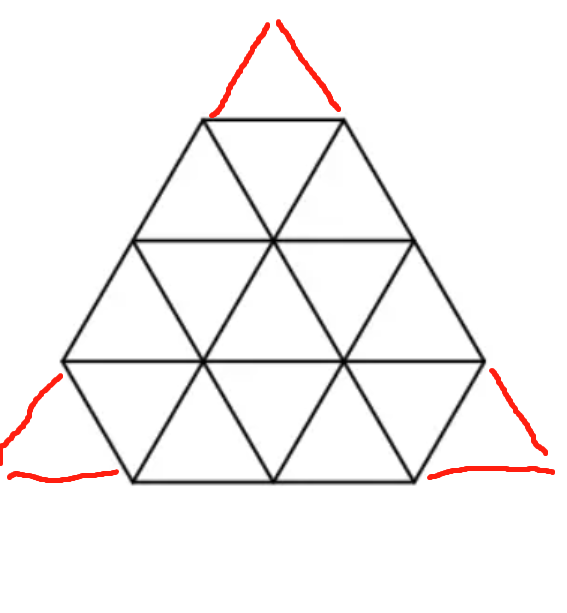
\includegraphics[width=0.86\linewidth]{assets/p7kRACD4cTf3YxK.png}\\[1pt]{\tiny\color{gray}\url{https://s2.loli.net/2023/08/17/p7kRACD4cTf3YxK.png}}\end{center}
  \item 正 $n$ 边形圆心角为 $\dfrac{360^{\circ}}{n}$ ，圆周角为 $\dfrac{180^{\circ}}{n}$ 。定义正 $n$ 边形上的三个顶点 $A,B$ 和 $C$（可以不相邻），使得 $\angle ABC=\theta$ ，当 $n\le 360$ 时，$\theta$ 可以取 $1^{\circ}$ 到 $179^{\circ}$ 间的任何一个整数 \href{https://codeforces.com/problemset/problem/1096/C}{See}。
  \item 某一点 $B$ 到直线 $AC$ 的距离公式为 $\dfrac{|\vec{BA}\times \vec{BC}|}{|AC|}$ ，等价于 $\dfrac{|aX+bY+c|}{\sqrt{a^2+b^2}}$。
  \item \texttt{atan(y / x)} 函数仅用于计算第一、四象限的值，而 \texttt{atan2(y, x)} 则允许计算所有四个象限的正反切，在使用这个函数时，需要尽量保证 $x$ 和 $y$ 的类型为整数型，如果使用浮点数，实测会慢十倍。
  \item 在平面上有奇数个点 $A_0,A_1,\dots,A_n$ 以及一个点 $X_0$ ，构造 $X_1$ 使得 $X_0,X_1$ 关于 $A_0$ 对称、构造 $X_2$ 使得 $X_1,X_2$ 关于 $A_1$ 对称、……、构造 $X_j$ 使得 $X_{j-1},X_j$ 关于 $A_{(j-1)\mod n}$ 对称。那么周期为 $2n$ ，即 $A_0$ 与 $A_{2n}$ 共点、$A_1$ 与 $A_{2n+1}$ 共点 \href{https://codeforces.com/contest/24/problem/C}{See} 。
  \item 已知 $A\ (x_A, y_A)$ 和 $X\ (x_X,y_X)$ 两点及这两点的坐标，构造 $Y$ 使得 $X,Y$ 关于 $A$ 对称，那么 $Y$ 的坐标为 $(2\cdot x_A-x_X,2\cdot y_A-y_X)$ 。
  \item \textbf{海伦公式}：已知三角形三边长 $a,b$ 和 $c$ ，定义 $p=\dfrac{a+b+c}{2}$ ，则 $S_{\triangle}=\sqrt{p(p-a)(p-b)(p-c)}$ ，在使用时需要注意越界问题，本质是铅锤定理，一般多使用叉乘计算三角形面积而不使用该公式。
  \item 棱台体积 $V=\frac{1}{3}(S_1+S_2+\sqrt{S_1S_2})\cdot h$，其中 $S_1,S_2$ 为上下底面积。
  \item 正棱台侧面积 $\frac{1}{2}(C_1+C_2)\cdot L$，其中 $C_1,C_2$ 为上下底周长，$L$ 为斜高（上下底对应的平行边的距离）。
  \item 球面积 $4\pi r^2$，体积 $\frac{4}{3}\pi r^3$。
  \item 正三角形面积 $\dfrac{\sqrt 3 a^2}{4}$，正四面体面积 $\dfrac{\sqrt 2 a^3}{12}$。
  \item 设扇形对应的圆心角弧度为 $\theta$ ，则面积为 $S=\frac{\theta}{2}\cdot R^2$ 。
\end{itemize}
\par\addvspace{2pt}\noindent\textbf{立体几何结论归档}\par
\begin{itemize}
  \item 已知向量 $\vec{r}=\{x,y,z\}$ ，则该向量的三个方向余弦为 $\cos \alpha =\dfrac{x}{|\vec r|}=\dfrac{x}{\sqrt{x^2+y^2+z^2}}; \ \cos \beta = \dfrac{y}{|\vec r|};\ \cos \gamma =\dfrac{z}{|\vec r|}$ 。其中 $\alpha,\beta,\gamma\in [0,\pi]$ ，$\cos^2\alpha+\cos^2\beta+\cos^2\gamma=1$ 。
\end{itemize}
